\chapter{Overview of the results and future prospects}\label{ch:overview}

The full analysis setup and the branching fraction measurement results in 
\Cref{sec:partial_branching_fraction_results,sec:total_branching_fraction_results}
are the ultimate goal of this analysis.
They represent the first implementation of an inclusive radiative analysis at Belle~II.
Moreover, it is the first implementation of a hadronic-tagged \BtoXsgamma measurement since 2007, 
when the result was reported by the BaBar collaboration (see \Cref{tab:btosgamma_inclusive_summary}).
The results of this Belle~II analysis are available in Ref.~\cite{Belle-II:2022hys}.

This Chapter is dedicated to the discussion and overview of the results, as well as their significance.
The prospects of \BtoXsgamma, focusing on the hadronic-tagged measurements, are also discussed.

\section{Discussion of the Belle~II hadronic-tagged \texorpdfstring{\BtoXsgamma}{B->Xs gamma} results}\label{sec:result_discussion}

The resulting values in \Cref{tab:integrated_branching_fractions} are in perfect agreement with the \SM predictions (see \Cref{sec:btosgamma_totalrate_theory}).
They also agree with the past measurements of \BtoXsgamma, which utilise both inclusive and sum-of-exclusive methods.
The visual comparison of all inclusive measurements is provided in \Cref{fig:measurement_comparison}.
\begin{figure}[htbp!]
    \centering
    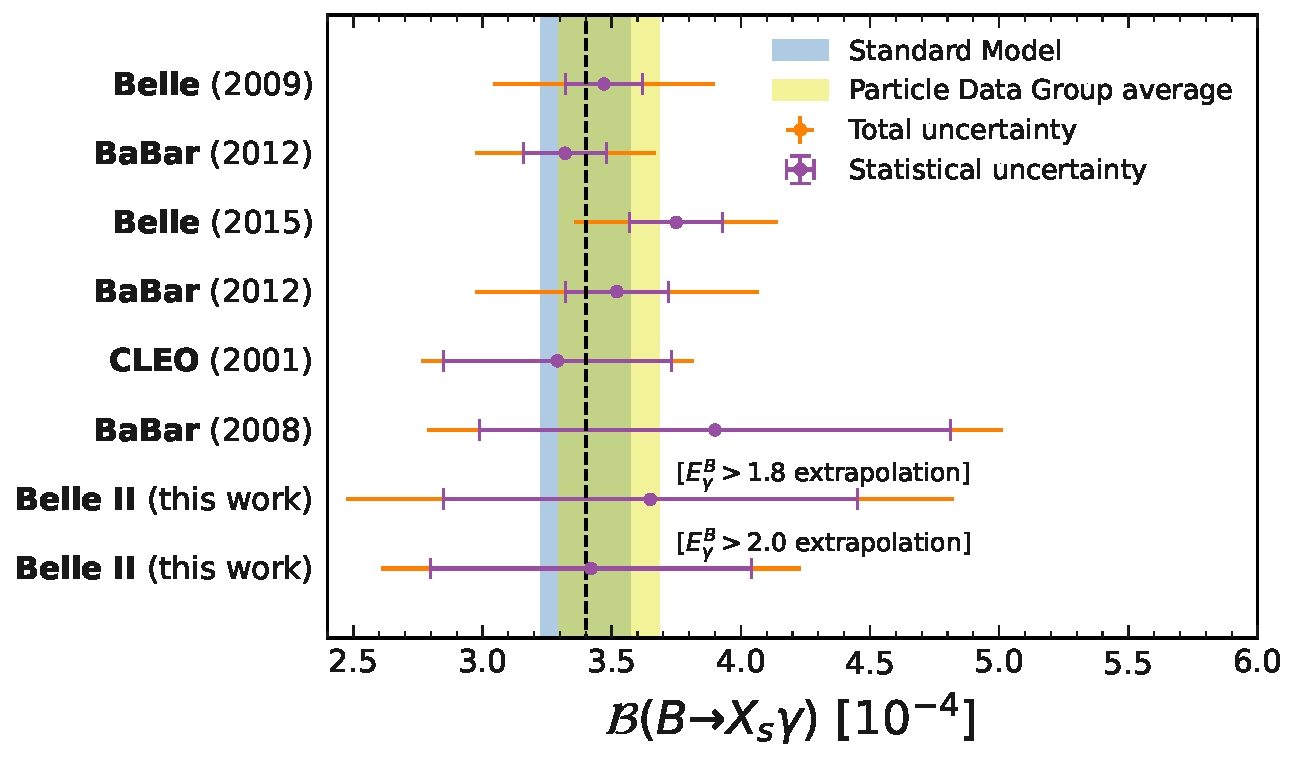
\includegraphics[width=0.5\textwidth]{figures/results_discussion/all_measurements_compared.pdf}
    \caption{\label{fig:measurement_comparison}
        The results of the measurement of the \BtoXsgamma branching fractions compared with past results from other experiments.
        The results from other experiments correspond to those in \Cref{tab:btosgamma_inclusive_summary}.
        The results from this analysis are taken from \Cref{tab:integrated_branching_fractions}.
        All values are at their extrapolated values (at $1.6~\gev$ lower energy threshold).
        The Standard Model expectation corresponds to the \Cref{eq:btosgamma_theoretical},
        whereas the Particle Data Group average to \Cref{eq:btosgamma_experimental}.
    }
\end{figure}

The hadronic-tagged \BtoXsgamma analysis uncertainty is dominated by its statistical component as seen in \Cref{tab:integrated_branching_fractions}.
The systematic uncertainty is larger than the statistical uncertainty only if the lowest-\EB signal-region interval is included in the integrated branching fraction evaluation, 
as the systematic uncertainty is driven by the number of background events in the post-fit sample.

Judging from the partial branching fractions of \BtoXsgamma in \Cref{sec:partial_branching_fraction_results},
the largest contribution to the systematic uncertainty originates from background modelling.
This contribution drops off quickly as the number of background events decreases.
The \Mbc fitting model uncertainties also drop quickly with \EB, as the main fitting difficulties originate from the contamination of \Mbc distribution by peaking non-\BtoXsgamma events.
On the other hand, the uncertainties due to signal modelling and \BtoXdgamma increase with \EB, as the number of \BtoXsdgamma events grows.

As discussed in \Cref{sec:btosgamma_techniques}, different analysis procedures are complementary to each other.
Therefore, although individually the result of this thesis is not competitive with the most precise measurements of BaBar and Belle (whose measurements are performed with up to 3 times larger datasets),
it demonstrates important consistency between different measurement techniques.
Furthermore, it is the second-ever measurement of the hadronic-tagged \BtoXsgamma: therefore it serves as proof of the measurement technique and its applicability across different experimental setups.

Consider the hadronic-tagged measurement of BaBar \cite{BaBar:2007yhb} (extrapolated to 1.6~\gev), which obtains:
\begin{equation}\label{eq:babar_measurement}
    \mathcal{B}(\BtoXsgamma) = (3.90 \pm 0.91 \mathrm{(syst.)} \pm 0.64 \mathrm{(stat.)}) \times 10^{-4}.
\end{equation}
It is possible to compare this to the results of the analysis presented here (\Cref{tab:integrated_branching_fractions})
to see that the statistical uncertainty of the Belle~II result is $0.91/0.80\approx1.14$ times lower.
The improvement of the statistical uncertainty is a combination of several reasons that include:
\begin{itemize}
    \item A higher tagging efficiency at Belle~II offered by the \FEI algorithm compared to the one used at BaBar (compare \FEI efficiency in \Cref{eq:tag_efficiency_with_uncertainty} with the 0.3\% reported in Ref.~\cite{BaBar:2007yhb});
    \item Different continuum suppression strategy (the Belle~II analysis uses a \BDT, whereas BaBar used a Fischer discriminant);
    \item Different fitting setup (the Belle~II analysis uses three \PDF{s}, whereas BaBar perform the fit using a Crystal Ball and ARGUS \PDF combination);
\end{itemize}

The systematic uncertainty highly depends on the lower-\EB threshold.
Therefore, a meaningful comparison is only such where the \EB threshold is the same.
The BaBar measurement in \Cref{eq:babar_measurement} is evaluated with a threshold of $\EB>1.9~\gev$.
The result of this analysis, evaluated at $1.8$ and $2.0$~\gev thresholds, can be approximated by linearly interpolating: $0.5\cdot(0.52+0.86)\approx0.69$.
Therefore, the systematic uncertainty is slightly higher but comparable, which is consistent with the lower-\EB threshold setting.
Furthermore, the evaluated uncertainties leave room for future improvement as will be discussed in \Cref{sec:future_prospects}.

Finally, the measurement of \EB distribution moments agrees well with the world average values \cite{Workman:2022ynf}:
\begin{equation}
    \expval{\EB} = 2.314 \pm 0.011 ~\gev; \quad \expval{\EB^2} - \expval{\EB}^2 = 0.303 \pm 0.0025.
\end{equation}
The uncertainties of the measured moments in \Cref{tab:moments} are several times larger than the world average values.
They contain a comparable significant statistical and systematic uncertainty component.

Interestingly, at higher-\EB thresholds (e.g. 2.1~\gev), while still larger, the systematic uncertainty is comparable to the total uncertainty of the world average.
Interpreting the uncertainties from the partial branching fraction measurement in \Cref{tab:partial_branching_fractions} indicates that background and fit modelling uncertainties are large contributors to the systematic uncertainty at lower-\EB thresholds.
Therefore, for improved accuracies of the hadronic tagged measurement,
the upcoming larger Belle~II dataset will not be sufficient alone:
parameter estimation, background subtraction and modelling uncertainties have to be further studied.
The next Section discusess the anticipated prospects for this goal.

\section{Future prospects for hadronic-tagged \safeBtoXsgamma analysis at Belle~II}\label{sec:future_prospects}

Belle~II is an ongoing experiment, which means that more and more \epem collision data will be recorded in the next decade.
No other ongoing experiment can contribute to the inclusive radiative measurements.
As it is clear from \Cref{sec:results} and \Cref{sec:result_discussion}, at the moment the analysis is limited by the statistical uncertainty.
With the larger Belle~II dataset, the importance of systematic effects will grow.
Although in this analysis several systematic uncertainties are set at their conservative estimates (see \Cref{sec:background_normalisation_systematic}, \Cref{sec:xdgamma_systematic} etc.),
additional studies will allow reducing them.
This was studied (as part of the original work for this thesis), and the results are available in Ref.~\cite{Belle-II:2022cgf}.
The uncertainty projections for the hadronic-tagged \BtoXsgamma are summarised in \Cref{tab:btosgamma_projections}.

\begin{table}[htbp!]
    \caption{\label{tab:btosgamma_projections}
    The projected uncertainties for the hadronic-tagged \BtoXsgamma with the increased Belle~II data set size.
    These projections are evaluated assuming the principal contributions in systematic uncertainty arise from
    background modelling and suppression uncertainties.
    The baseline case is presented for a scenario where the remaining good tag-\B meson background is known to $10\%$,
    whereas the improved scenario corresponds to where it is known to a $5\%$ accuracy.
    }
    \begin{tabular}{|ccccc|c|}
        \hline
        \multirow{2}{*}{Lower \EB threshold} & \multicolumn{4}{c}{Statistical uncertainty} & \multirow{2}{*}{\makecell{Baseline (improved)\\ systematic uncertainty}} \\
        & 1~\invab& 5~\invab & 10~\invab & 50~\invab & \\
        \hline
        1.4~\gev & 10.7\% & 6.4\% & 4.7\% & 2.2\% & 10.3 \% (5.2\%)\\
        1.6~\gev & 9.9 \% & 6.1\% & 4.5\% & 2.1\% & 8.5 \% (4.2\%)\\ 
        1.8~\gev & 9.3 \% & 5.7\% & 4.2\% & 2.0\% & 6.5 \% (3.2\%)\\ 
        2.0~\gev & 8.3 \% & 5.1\% & 3.8\% & 1.7\% & 3.7 \% (1.8\%)\\ 
        \hline
    \end{tabular}
\end{table}

The statistical uncertainties for the hadronic tagged \BtoXsgamma are expected to reach $5\%$ level with $5~\invab$ of Belle~II data.
The systematic uncertainty expectations are evaluated assuming that the main contributor to the systematic uncertainty
is the remaining-\BB background subtraction and \FEI tagging.
If the knowledge of remaining-\BB background stays at the 10\% level ($8.7\%$ evaluated in this analysis) and \FEI calibration uncertainty is not improved,
it is expected that a 6.5\% total systematic uncertainty on the branching fraction of \BtoXsgamma can be achieved.
On the other hand, if remaining after-fit \BB background modelling is understood to a $5\%$ level it is plausible to half the expected systematic uncertainty.
The uncertainties on signal selection efficiency will further reduce as the understanding of background suppression tools (e.g. the \piz veto, \ZMVA) improves.
The \BtoXdgamma component will be accurately subtracted when precise \BtoXdgamma measurements with Belle~II are performed.


Summarising, world-leading hadronic-tagged \BtoXsgamma measurements with Belle~II datasets of $1-5~\invab$ are possible if remaining background contributions are understood to a 5\% or higher precision.
This is an important observation given the fact that other types of inclusive \BtoXsgamma analysis techniques with the Belle and BaBar datasets are already limited by systematic uncertainties (see \Cref{tab:btosgamma_inclusive_summary}).
Therefore, a different approach, one that will be provided by the hadronic-tagged analyses, is necessary for further insights into the radiative \BtoXsgamma transitions.
In the shorter term, as Belle has not reported a hadronic-tagged \BtoXsgamma analysis, a joint Belle and Belle~II analysis may provide a total dataset of approximately $1\invab$, enabling such results in the next couple of years.

\section{Input of the results to the SIMBA global fit}\label{sec:input_to_theory}

In a collaborative effort with the SIMBA collaboration, the results of \Cref{tab:partial_branching_fractions}
have been used to evaluate the $m_b$ and $\lambda_1$ and the $\mathcal{C}_7^{\mathrm{incl}}$ parameters (see \Cref{sec:btosgamma_spectrum_theory}). 
Originally in Ref.~\cite{Bernlochner:2020jlt}, a simultaneous parameter estimation fit is performed using all available experimental results of the photon energy spectrum that include
BaBar and Belle results of hadronic, sum-of-exclusive, lepton-tagged and untagged measurement strategies.
The same procedure in terms of the fitting strategy is repeated with the additional Belle~II result described in this thesis.

The fit results and the comparison of the effect on the estimated value and uncertainties of the fit parameters are shown in \Cref{fig:simba_c7}.
Note that the $\EB\in(1.8,2.0)~\gev$ interval of the Belle~II result is excluded from the fit due to the large uncertainty and differences in the interval widths compared to earlier \BtoXsgamma measurements.
The results slightly shift the central values of the parameters but the overall result retains a similar uncertainty and is consistent with the earlier results.
\begin{figure}[htbp!]
    \centering
    \subcaptionbox{\label{fig:simba_fit}}{
        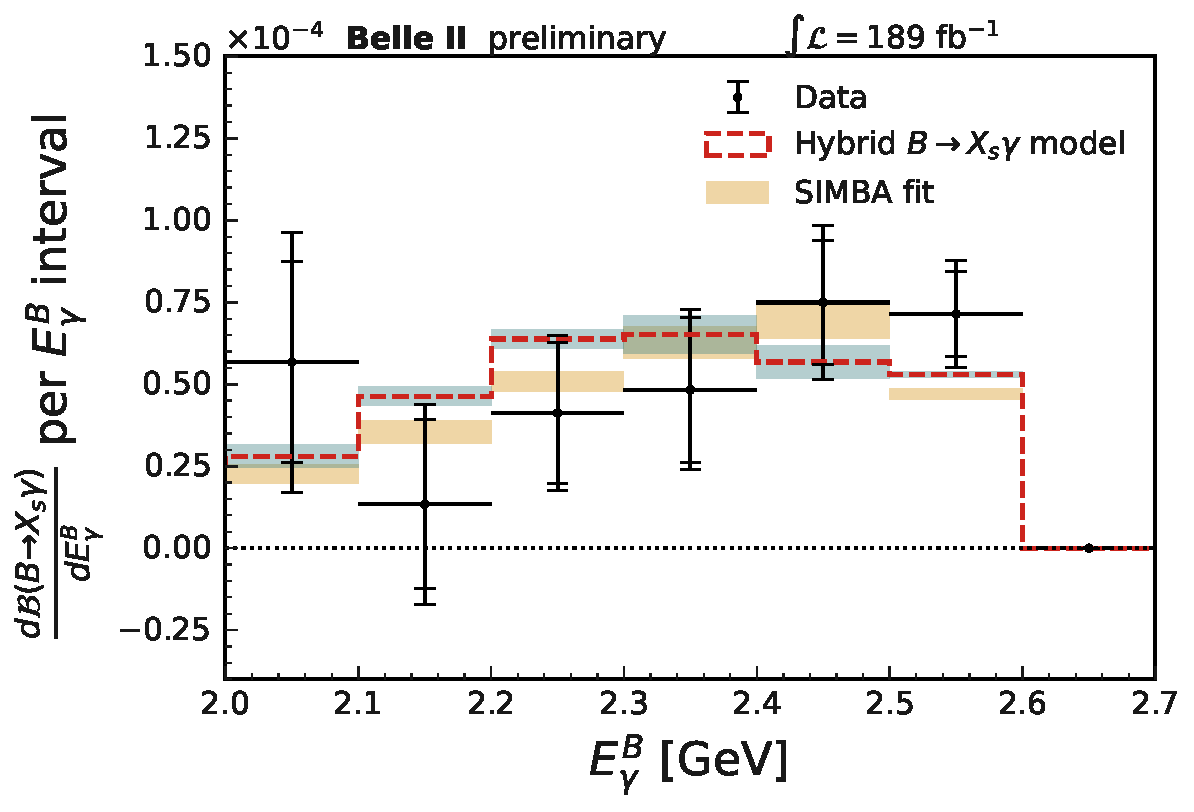
\includegraphics[width=0.45\textwidth]{figures/results_discussion/simba_partial_bfs_expectation.pdf}
    }
    \subcaptionbox{\label{fig:c7}}{
        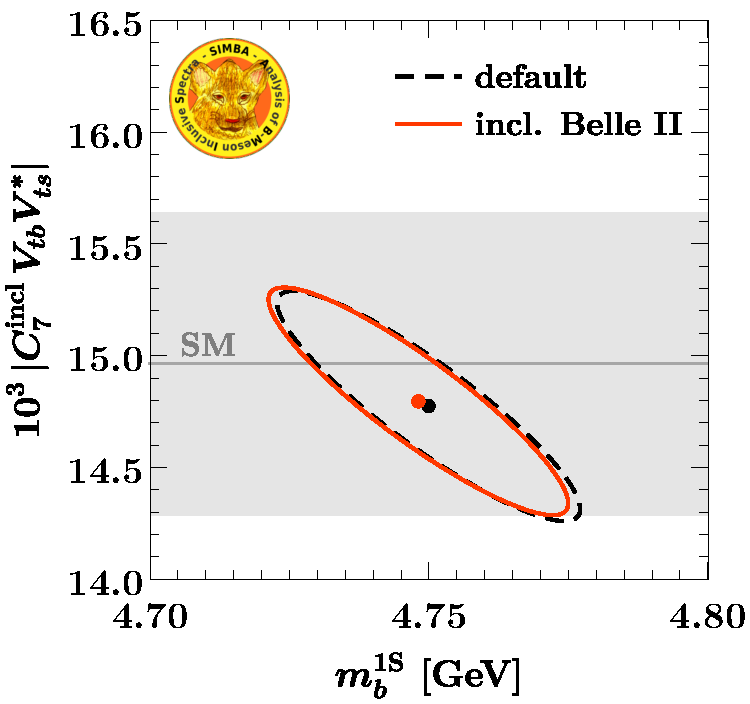
\includegraphics[width=0.4\textwidth]{figures/results_discussion/C7incl_mb_la055_henrikas.pdf}
    }
    \caption{\label{fig:simba_c7}
    The results of the \BtoXsgamma spectrum parameter determination by the SIMBA collaboration which includes the results of the work presented in this thesis
    \cite{Bernlochner:2020jlt}.
    \Cref{fig:simba_fit} shows the results of the SIMBA fit superimposed on \Cref{fig:partial_branching_fraction}.
    \Cref{fig:c7} shows the corresponding $|C^{\mathrm{incl}}_7V^{}_{tb}V^*_{ts}|$ and $m_b^{1S}$ values.
    The dark dashed line (default) corresponds to the result without the Belle~II results, whereas the red curve demonstrates the result with the Belle~II results included.
    As expected due to the current low statistical precision of the added \BtoXsgamma measurement of Belle~II, the impact is small.
    Credit to the SIMBA collaboration for the values and \Cref{fig:c7}.
    }
\end{figure}


With the new inputs from Belle~II, the determined SIMBA values are:
\begin{equation}\label{eq:new_simba_values}
    m_b^{1S}= 4.748\pm0.043~\gevcc; \quad \lambda_1^{\mathrm{inv}} = -0.219\pm0.082~\gev^2/c^4,
\end{equation}
where the results can be directly compared with the previous values from SIMBA given in \Cref{eq:simba_result}.
The uncertainties for both values, as before, combine fitting, theoretical and parametric components.
The latter two are assumed to not change when evaluating the total uncertainty.
While the current impact of the Belle~II results is small, the results of the hadronic-tagged Belle~II analyses still have room for improvement, as discussed in \Cref{sec:future_prospects}.
Moreover, they provide better sensitivity to the details of the \EB spectrum, due to the direct access to the $B$ meson rest frame.
Therefore, future versions of the Belle~II analysis presented in this thesis will be key inputs to the SIMBA results and other global fits, such as Ref.~\cite{Haller:2018nnx}.